\documentclass[12pt,a4paper]{article}
\usepackage[utf8]{inputenc}
\usepackage[english]{babel}

\usepackage{amsmath}
\usepackage{amsfonts}
\usepackage{amssymb}

\usepackage{graphicx}
\usepackage{caption}
\usepackage{subcaption}
\usepackage{lmodern}
\usepackage{tikz}
\usepackage{titlesec}
\usepackage{environ}
\usepackage{xcolor}
\usepackage{fancyhdr}
\usepackage[colorlinks = true, linkcolor = black]{hyperref}
\usepackage{xparse}
\usepackage{enumitem}
\usepackage{comment}
\usepackage{wrapfig}
\usepackage[capitalise]{cleveref}

\usepackage[left=2cm,right=2cm,top=2cm,bottom=2cm]{geometry}
\usepackage{multicol}
\usepackage[indent=0pt]{parskip}

\newcommand{\spaceP}{\vspace*{0.5cm}}
\newcommand{\Span}{\mathrm{Span}\,}
\newcommand{\range}{\mathrm{range}\,}
\newcommand{\ra}{\rightarrow}

%% Redefining sections
\newcommand{\sectionformat}[1]{%
    \begin{tikzpicture}[baseline=(title.base)]
        \node[rectangle, draw] (title) {#1};
    \end{tikzpicture}
    
    \noindent\hrulefill
}

\newif\ifhNotes 

\hNotesfalse

\ifhNotes
	\newcommand{\hideNotes}[1]{%
	\phantom{#1}
	}
	\newcommand{\hideNotesU}[1]{%
	\underline{\hspace{1mm}\phantom{#1}\hspace{1mm}}
	}
\else
	\newcommand{\hideNotes}[1]{#1}
	\newcommand{\hideNotesU}[1]{\textcolor{blue}{#1}}
\fi

% default values copied from titlesec documentation page 23
% parameters of \titleformat command are explained on page 4
\titleformat%
    {\section}% <command> is the sectioning command to be redefined, i. e., \part, \chapter, \section, \subsection, \subsubsection, \paragraph or \subparagraph.
    {\normalfont\large\scshape}% <format>
    {}% <label> the number
    {0em}% <sep> length. horizontal separation between label and title body
    {\centering\sectionformat}% code preceding the title body  (title body is taken as argument)

%% Set counters for sections to none
\setcounter{secnumdepth}{0}

%% Set the footer/headers
\pagestyle{fancy}
\fancyhf{}
\renewcommand{\headrulewidth}{0pt}
\renewcommand{\footrulewidth}{2pt}
\lfoot{P.-O. Paris{\'e}}
\cfoot{MATH 241}
\rfoot{Page \thepage}

%% Defining example environment
\newcounter{example}[section]
\NewEnviron{example}%
	{%
	\noindent\refstepcounter{example}\fcolorbox{gray!40}{gray!40}{\textsc{\textcolor{red}{Example~\theexample.}}}%
	%\fcolorbox{black}{white}%
		{  %\parbox{0.95\textwidth}%
			{
			\BODY
			}%
		}%
	}

% Theorem environment
\NewEnviron{theorem}%
	{%
	\noindent\refstepcounter{example}\fcolorbox{gray!40}{gray!40}{\textsc{\textcolor{blue}{Theorem~\theexample.}}}%
	%\fcolorbox{black}{white}%
		{  %\parbox{0.95\textwidth}%
			{
			\BODY
			}%
		}%
	}

\NewEnviron{notes}%
	{%
	\noindent \fcolorbox{gray!40}{gray!40}{\textsc{\textcolor{blue}{Solution.}}}%
	%\fcolorbox{black}{white}%
		{  %\parbox{0.95\textwidth}%
			{
			\textcolor{blue}{%
			\BODY
			}
			}%
		}%
	}
%%% Ignorer les notes
\excludecomment{notes}

%%%%
\begin{document}
\thispagestyle{empty}

\begin{center}
\vspace*{2.5cm}

{\Huge \textsc{Math 241}}

\vspace*{2cm}

{\LARGE \textsc{Chapter 4}} 

\vspace*{0.75cm}

\noindent\textsc{Section 4.2: Definite Integral}

\vspace*{0.75cm}

\tableofcontents

\vfill

\noindent \textsc{Created by: Pierre-Olivier Paris{\'e}} \\
\textsc{Fall 2022}
\end{center}

\section{General Definition}

Suppose we have a region $S$ under the graph of a function $y= f(x)$ from $x = a$ to $x = b$.

	\begin{center}
	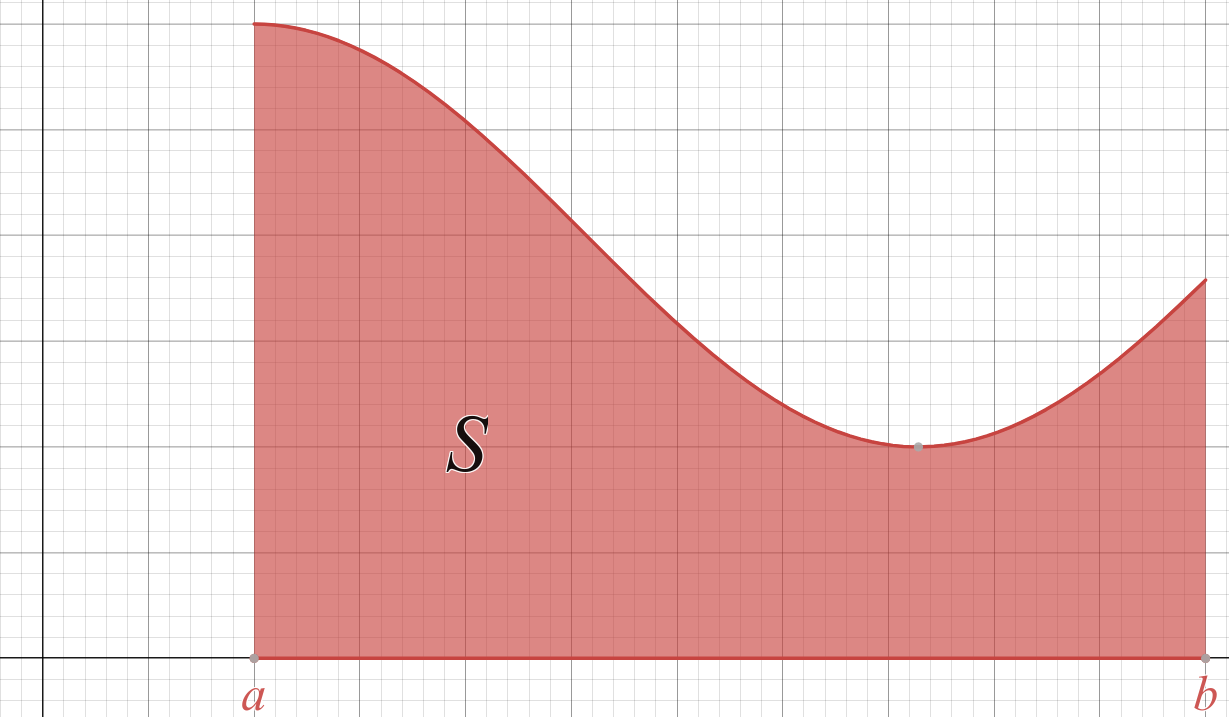
\includegraphics[scale=0.39]{regionS.png}
	\end{center}
	
\textbullet Divide the interval $[a, b]$ in $n$ subintervals of equal length $\Delta x = (b - a)/n$.

	\begin{center}
	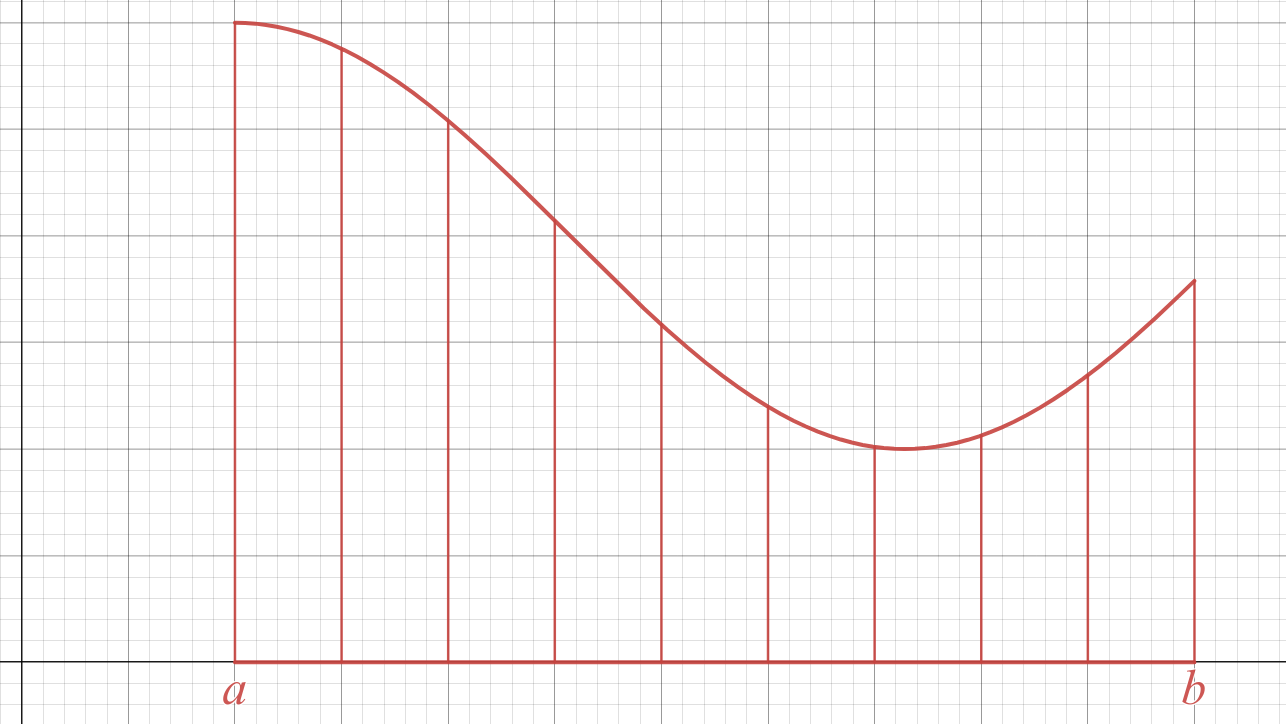
\includegraphics[scale=0.37]{regionSDivided.png}
	\end{center}
	
\textbullet Select some number $x_i^\ast$ in each $[x_{i-1}, x_{i}]$ (can be any number within the subinterval).

\textbullet Form the sum: $\displaystyle S_n = \sum_{i = 1}^{n} f (x_i^{\ast}) \Delta x = f(x_1^{\ast}) \Delta x + f(x_2^\ast) \Delta x + \cdots + f (x_{n}^\ast) \Delta x .$

\newpage

\underline{Definite Integral:} For a continuous function $f$, the definite integral of $f$ is defined by
	\begin{align*}
	\int_a^b f (x) \, dx = \lim_{n \ra \infty} S_n = \lim_{n \ra \infty} \Big( \sum_{i = 1}^{n} f (x_i^{\ast}) \Delta x \Big) .
	\end{align*}
	
\underline{Important Remarks:}
	\begin{itemize}
	\item Description of the terminology:
		\begin{itemize}
		\item Symbol $\displaystyle \int$:
		\item $a$: 
		\item $b$:
		\item $f(x)$: 
		\item $dx$: 
		\end{itemize}
	\item The definite integral is a \textbf{number}! It does not depend on $x$! This means that
		\begin{align*}
		\int_a^b f(x) \, dx = \int_a^b f(r) \, dr = \int_a^b f(t) \, dt = \ldots
		\end{align*}
	\item The expression $S_n$ are called \textbf{Riemann Sums}.
	\item When $f(x) \geq 0$, then $\displaystyle\int_a^b f(x) \, dx$ is the area of the region $S$:
		\begin{align*}
		\mathrm{Area}(S) = \int_a^b f(x) \, dx .
		\end{align*}
	\item If $f(x)$ is negative somewhere, then $\displaystyle \int_a^b f(x) \, dx$ is the \textbf{net area} between the graph of $y = f(x)$ and the horizontal line $y = 0$ (the $x$-axis).
		\begin{center}
		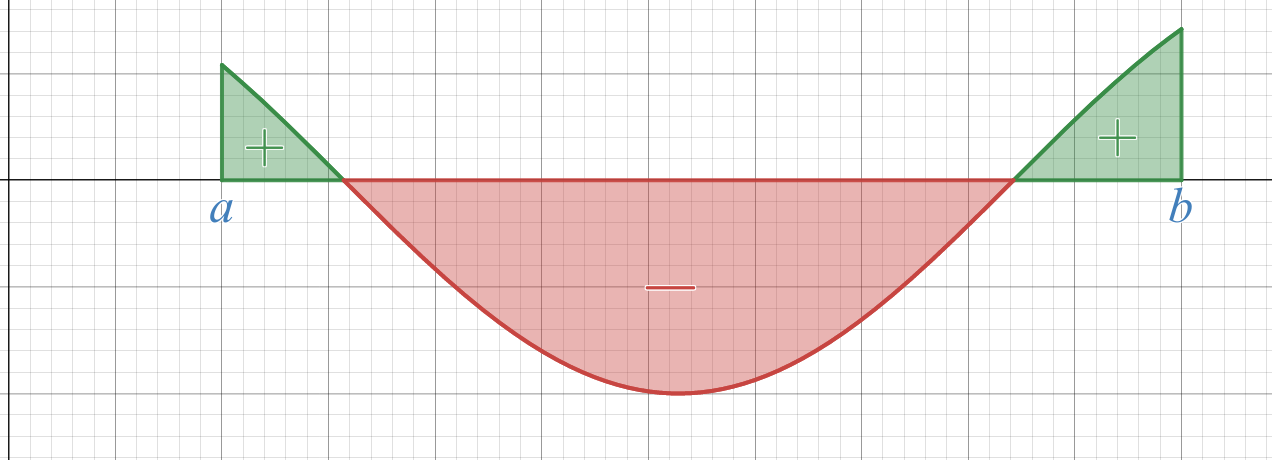
\includegraphics[scale=0.35]{NetArea.png}
		\end{center}
	\end{itemize}
	
	\newpage
	
	\begin{example}
	Find the value of the following integrals.
		\begin{multicols}{4}
		\begin{enumerate}[label=\textbf{(\alph*)}]
		\item $\displaystyle \int_0^1 x \, dx$.
		\item $\displaystyle \int_{-1}^1 x \, dx$.
		\item $\displaystyle \int_0^2 |x - 1| \, dx$.
		\end{enumerate}
		\end{multicols}
	\end{example}
	
	\vfill
	
	\underline{Useful Trick:} Try to intepret the integral geometrically!
	
	\newpage
	
	\section{Properties of The Definite Integral}
	
	\subsection{Playing with Lower and Upper Bounds}
	\begin{itemize}
	\item If we change the order of the lower and upper bounds, then
		\begin{align*}
		\int_b^a f(x) \, dx = - \int_a^b f(x) \, dx .
		\end{align*}
	\item If the lower and upper bounds are equal, the definite integral is zero, that is
		\begin{align*}
		\int_a^a f(x) \, dx = 0 .
		\end{align*}
	\end{itemize}
	
	\vspace*{16pt}
	
	\underline{Illustration:}
	
	\begin{center}
		\begin{tikzpicture}
			\draw[black, very thick, >=latex, ->] (-0.2, 0) -- (13,0)node[below]{$x$};
			\draw[black, very thick, >=latex, ->] (0, -0.2) -- (0, 8.5)node[left]{$y$};
		\end{tikzpicture}
	\end{center}
	
	\subsection{Algebraic operations}
	For two continuous functions $f(x)$ and $g(x)$ on the interval $[a, b]$,
	\begin{itemize}
	\item \underline{Addition}: $\displaystyle \int_a^b (f (x) + g(x)) \, dx = \int_a^b f(x) \, dx + \int_a^b g(x) \, dx$.
	\item \underline{Substraction:} $\displaystyle \int_a^b (f (x) - g(x)) \, dx = \int_a^b f(x) \, dx - \int_a^b g(x) \, dx$.
	\item \underline{Multiplication by constant}: $\displaystyle \int_a^b c f(x) \, dx = c \int_a^b f(x) \, dx$.
	\end{itemize}
	
	\newpage
	
	\subsection{Useful Formulas}
	Go to Desmos: \url{https://www.desmos.com/calculator/mr9ba23hpz}.
		\begin{multicols}{2}
		\begin{itemize}
		\item $\displaystyle\int_a^b 1 \, dx = $
		\item $\displaystyle\int_a^b x \, dx = $
		\end{itemize}
		\end{multicols}
		%\begin{center}
		%\begin{tikzpicture}
		%	\draw[black, very thick, >=latex, ->] (-8, 0) -- (0, 0)node[below]{$x$};
		%	\draw[black, very thick, >=latex, ->] (-4, -3.5) -- (-4, 3.5)node[left]{$y$};
		%	\draw[black, very thick, >=latex, ->] (1, 0) -- (9, 0)node[below]{$x$};
		%	\draw[black, very thick, >=latex, ->] (5, -3.5) -- (5, 3.5)node[left]{$y$};`
		%\end{tikzpicture}
		%\end{center}
	\begin{itemize}
	\item In general,
		\begin{align*}
		\int_a^b x^n \, dx = \phantom{\frac{b^{n+1} - a^{n+1}}{n + 1} 222222} .
		\end{align*}
	\end{itemize}
	
	\begin{example}
	Using the properties of the integral and the formulas, find the value of the following integrals.
		\begin{enumerate}[label=\textbf{(\alph*)}]
		\item $\displaystyle \int_0^1 2x^2 - x^4 \, dx$.
		\item $\displaystyle \int_{-2}^2 4x^4 - 3 x^2 \, dx$.
		\end{enumerate}
	\end{example}
	
	\newpage
	
	\subsection{Cutting the domain}
	Let $a < c < b$ and $f(x)$ be a continuous function on $[a, b]$. Then
		\begin{align*}
		\int_a^b f(x) \, dx = \int_a^c f(x) \, dx + \int_c^b f (x) \, dx .
		\end{align*}
	
	\underline{Illustration:}
	
	\begin{center}
		\begin{tikzpicture}
			\draw[black, very thick, >=latex, ->] (-0.2, 0) -- (13,0)node[below]{$x$};
			\draw[black, very thick, >=latex, ->] (0, -0.2) -- (0, 8.5)node[left]{$y$};
		\end{tikzpicture}
	\end{center}
	
	\vspace*{16pt}
		
	\begin{example}
	If it is known that $\displaystyle \int_0^{10} f(x) \, dx = 17$ and $\displaystyle \int_0^8 f(x) \, dx = 12$, then find $\int_8^{10} f(x) \, dx$.
	\end{example}
	
	\newpage
	
	\subsection{Comparison Properties}
	\begin{itemize}
	\item If $f(x) \geq 0$ for $a \leq x \leq b$, then $\displaystyle \int_a^b f(x) \, dx \geq 0$.
	\item If $f(x) \geq g(x)$ for $a \leq x \leq b$, then $\displaystyle \int_a^b f(x) \, dx \geq \int_a^b g(x) \, dx$.
	\item If $m \leq f(x) \leq M$ for $a \leq x \leq b$, then
		\begin{align*}
		m (b - a) \leq \int_a^b f(x) \, dx \leq M (b - a) .
		\end{align*}
	\end{itemize}
	
	\vspace*{12pt}
	
	\begin{example}
	Use the last comparison property to estimate $\displaystyle \int_1^4 \sqrt{x} \, dx$.
	\end{example}

\end{document}